\documentclass[a4paper,12pt,titlepage]{report}

\usepackage[utf8]{inputenc}
\usepackage[T1]{fontenc}
\usepackage[french]{babel}
\usepackage{mathtools,amssymb,amsthm}
\usepackage[top=20mm, bottom=25mm, left=15mm, right=15mm]{geometry}
\usepackage{hyperref}
\usepackage{xcolor}

\newcommand{\octave}{\textit{Octave }}

\setcounter{secnumdepth}{3}
\renewcommand{\thesection}{\arabic{section}.}
\renewcommand{\thesubsection}{\arabic{section}.\arabic{subsection}}
%\titleformat{\subsubsection}[runin]{\normalfont\bfseries}{\thesubsubsection}{0em}{}

\usepackage{listings}
	\lstset{	
		basicstyle={\scriptsize},
		numbers={left},
		numbersep=5pt,
		backgroundcolor=\color{orange!10!white},
		frame=l,
		numberstyle=\tiny\color{red},
		breaklines=true,
		xleftmargin=10pt,
		framexleftmargin=1pt,
		keywordstyle=\bfseries\color{green!40!black},
	 	commentstyle=\itshape\color{blue!40!black},
	  	identifierstyle=\color{white!20!black},
	 	stringstyle=\color{orange}	 	
	 	}
\renewcommand{\lstlistingname}{Code}
\renewcommand{\lstlistlistingname}{Table des extraits de code}
\setlength{\parskip}{0.5em}

\title{Livrable supplémentaire Projet Signal\\Reconnaissance Optique de Caractères}
\author{Tristan DRUSSEL - Florian POUTHIER \\ \\ Génie Électrique - 4ème année\\ INSA Strasbourg}
\date{Année scolaire 2019-2020}

\begin{document}
	\begin{titlepage}
		\maketitle
	\end{titlepage}
	\tableofcontents
	\newpage
	\section{Introduction}
	Le présent rapport ne comprend que les éléments du livrable supplémentaire. Les principales fonctionnalités sont présentées dans le rapport d'avancement 2. Les précédents codes, sources et rapports sont disponible sur le dépôt Git du projet : \url{https://github.com/tristanplouz/ProjetSignal} \\
	Le livrable supplémentaire que nous avons décidé d'implémenter est la reconnaissance des couleurs et des styles. En effet reconnaitre du texte de toutes les couleurs mais ne pas pouvoir le retransmettre en couleur et avec des effets, c'est un peu triste, tout comme un ciel gris strasbourgeois ou un monde sans aucune couleur.
	Nous allons dans un premier temps parler de comment retransmettre un document en couleur et dans un second temps nous verrons comment détecter les styles et les couleurs.
	\section{Retransmission}
	Dans la partie suivante, nous allons parler de comment détecter les éléments hypertextuels, mais dans cette partie nous allons parler de comment les retransmettre.\\
	Nous avons besoin d'un format qui soit accessible et reproductible facilement. Lorsque l'on pense à des éléments colorés et stylisés, on pense premièrement à une image. Mais détecter du texte dans une image pur ensuite reproduire une image est un travail assez contre productif. Dans un second temps, nous pouvons penser à un fichier PDF contenant le texte stylisé. Cette technique n'est malheureusement pas simple à réaliser en ayant un PDF avec le texte accessible. La création d'un document PDF peut s'effectuer avec un traitement de texte, mais créer un fichier \texttt{.odt} n'est pas non plus simple. Nous pouvons penser à un compilateur \LaTeX{} mais encore une fois c'est un énorme outil pour une petite tâche. Pour stocker du texte, on pense au format textuel comme le \texttt{.txt} ou le \texttt{Markdown} malheureusement ces formats ne prennent pas en compte les effets stylistiques. Nous avons besoin d'un outil entre le simple fichier texte et le document de traitement texte au niveau de la complexité. Deux éléments peuvent alors apparaitre la syntaxe Wiki, cela permet de créer de gros document avec une structure et de la mise en forme, l'inconvénient est qu'il faut un interpréteur Wiki. On peut finalement arriver au \texttt{HTML}, ce langage de description textuel, permet de restituer des éléments textuels stylisés. De plus il est facilement interprétable, il suffit d'un simple navigateur. Couplé au \texttt{CSS}, il permet de réaliser tous les effets hypertextuels que nous souhaitons.
	\paragraph{HTML et CSS} Le \texttt{HTML} (Hyper Text Markup Language) et le \texttt{CSS} (Cascading Style Sheets) sont des langages de balisages et de mise en forme principalement utilisé sur l'internet. Le \texttt{HTML}, créé dans les années 1990, est un des premiers pas du Web tel qu'on le connais aujourd'hui. Le \texttt{CSS} se démocratise dans les années 2000. Si le \texttt{HTML} décrit le squelette et les informations du document, le \texttt{CSS} se charge de la mise en page. Aujourd'hui, d'autres standards se sont rajouter dans le milieu des pages WEB et les pages constituées à 100\% en HTML et CSS ne sont que des vestiges des années 2010.\newpage
	\paragraph{Application à notre sujet} Nous souhaitons réaliser une simple page qui reprend le texte décodé et les effets détecter.
\begin{lstlisting}[caption={Structure de base du HTML},language=HTML]
<!DOCTYPE html>
<html>
	<head>
		<title>Titre</title>
		<style>
		Style CSS
		</style>
	</head>
	<body>
	Corps du document
	</body>
</html>
\end{lstlisting}
	Afin de réaliser cela, notre code va créer des chaines de caractères comportant les balises \texttt{HTML} requises et en ajoutant des propriétés de style correspondantes.
	\section{Détection}
	Dans nos applications, nous laissons toujours le choix à l'utilisateur de ce qu'il souhaite. Nous demandons à l'utilisateur si il souhaite une sortie texte simple dans la console ou si il souhaite les éléments textuels et hypertextuels. Si le texte comprend des éléments hypertextuels mais que l'utilisateur à demander une sortie simple, il peut y avoir des erreurs de détection.
	\subsection{Couleurs}
	Dans un premier temps, nous allons voir comment nous détectons les couleurs. 
	\paragraph{Les couleurs} Les couleurs sont ici codées sur 3 octets représentant respectivement le rouge, le vert et le bleu. Ce système de couleur est donc cubique. Nous pouvons donc avoir 256 valeurs de rouge, de bleu et de vert, en les "mélangeant" nous pouvons donc obtenir $256*256*256=1.6777216\times 10^7$ couleurs. On travaille en synthèse additive, si on somme toutes les couleurs on obtient du blanc.\\
	Il existe en revanche d'autres système de codage des couleurs comme le CMY (Cyan, Magenta, Yellow) qui travaille en synthèse soustractive, si on somme toutes les couleurs on obtient du noir.\\ Ou encore le système HSL (Hue, Saturation, Luminance), où on travaille avec une teinte, une saturation et une luminosité, on ne travaille plus dans un cube mais dans un cone ou double cone.
	\paragraph{Traitement} Notre image est donc une matrice dont chaque élément, pixel, est représenté par son intensité en rouge, vert et en bleu. 
	\subparagraph{Arrière plan} Dans un premier temps, nous détectons la couleur de l'arrière plan en effet, elle sera utile par la suite. On considère que la couleur du fond est uniforme. Nous allons donc parcourir toute l'image et compter les occurrences de chaque couleur. On peut ensuite trouver la couleur la plus présente est en déduire que c'est la couleur de fond.  \\
	On l'inscrit ensuite dans la page \texttt{HTML}.
	\begin{lstlisting}[caption={Style pour le fond},language=HTML]
<style>
	body{
	 background:rgb(r,g,b);	
	}
</style>
\end{lstlisting}
\begin{lstlisting}[caption={Insertion de la couleur de fond dans Octave},language=Octave]
page=cstrcat("[..]<style>body{background:rgb(",num2str(colorBG(1)),",",num2str(colorBG(2)),",",num2str(colorBG(3)),");}</style>[..]");
\end{lstlisting}
	\subparagraph{Lettre} Ensuite, on détermine la couleur de chaque lettre, dans ce cas, on travaille sur nos tuiles. On effectue la même recherche sur notre tuile, en comptant chaque occurrence de couleur. On trouve ensuite la couleur la plus présente qui n'est pas la couleur de fond.\\
	Cette fois dans le code \texttt{HTML}, on injecte une balise de type \textsl{<span>} en lui définissant le style dans la balise.
	\begin{lstlisting}[caption={Insertion de la couleur de la lettre dans Octave},language=Octave]
predict=cstrcat("<span style='color:rgb(",num2str(colorL(1)),",",num2str(colorL(2)),",",num2str(colorL(3)),");'>",predict,"</span>");
\end{lstlisting}
	\paragraph{Optimisation}
	Parcourir toutes l'image pour chercher chaque couleur est une technique un peu longue et pas vraiment utile. C'est pour cela que l'on ne parcourt pas l'image dans son entièreté mais seulement une colonne et une ligne tous les x, ainsi on obtient une image où les proportions de couleurs sont respectées et donc on accélère le traitement.
	\begin{figure}[h]
	\centering
		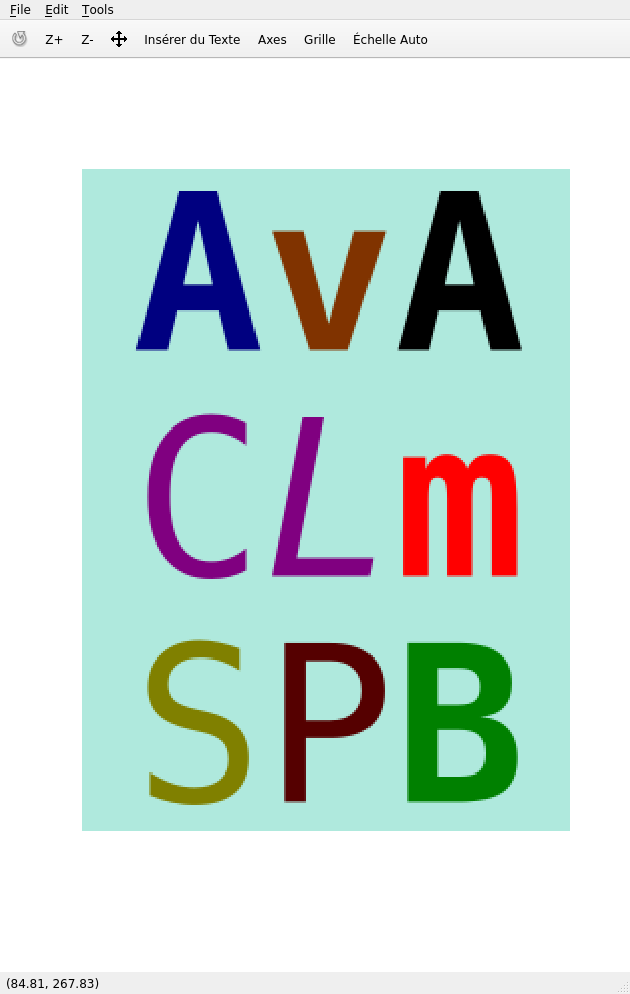
\includegraphics[width=0.25\textwidth]{../illus/1s1.png}
		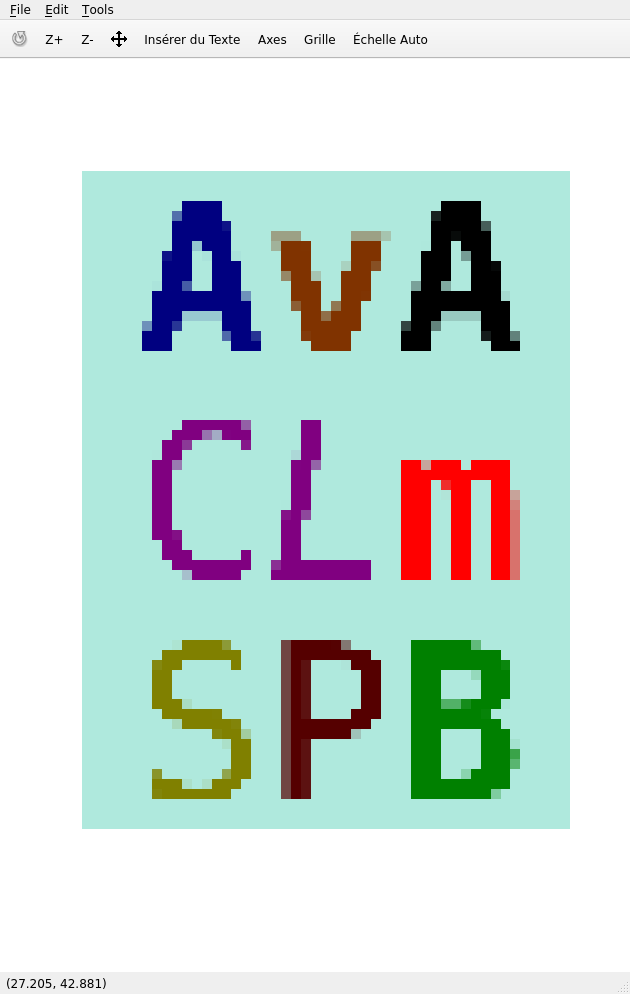
\includegraphics[width=0.25\textwidth]{../illus/1s5.png}
		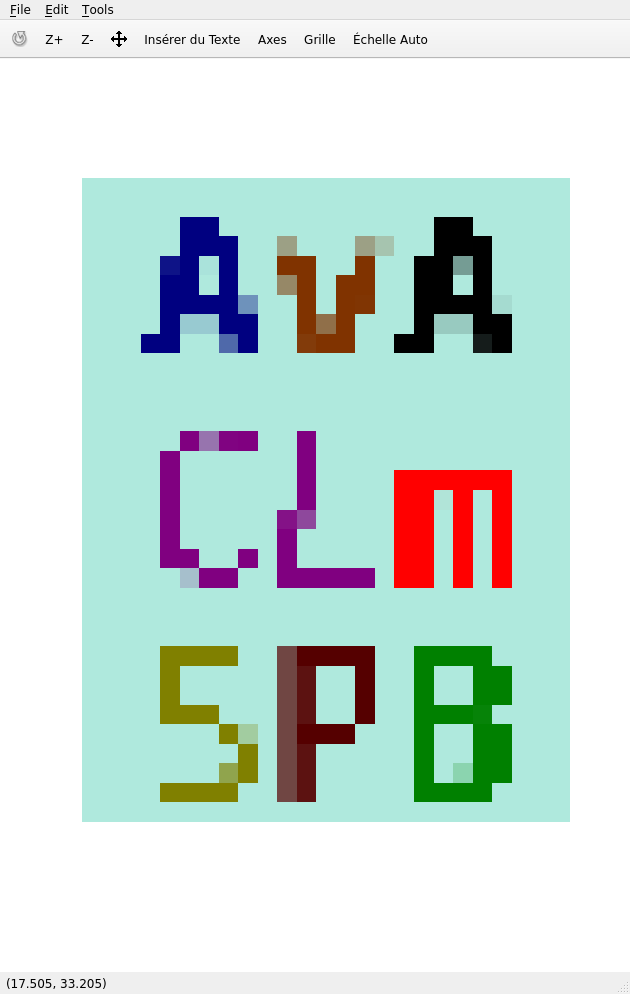
\includegraphics[width=0.25\textwidth]{../illus/1s10.png}
		\caption{Image en prenant: Toutes les lignes, 1 ligne sur 5 et 1 ligne sur 10}
	\end{figure}
	On prend donc 1 ligne sur 10 pour détecter la couleur de fond et une ligne sur 5 pour détecter la couleur de la lettre.
	\subsection{Gras}
	Pour détecter le \textbf{gras}, nous sommes partis du constat que la forme générale du caractère ne changeait pas, en effectuant des tests, nous pouvons nous apercevoir que le coefficient de corrélation ne diminue pas tant que ça et la lettre est encore détectable. Un point qui change est la surface d'occupation de la lettre sur la tuile, en effet une police grasse occupe plus de place qu'une police standard. Nous calculons donc le rapport d'occurrence de la couleur de lettre sur la couleur de fond pour la tuile mais aussi pour l'échantillon de notre base de données. Lorsque la police est grasse, on a un rapport plus élevé. En calculant le rapport de l’échantillon et de la tuile, on peut déterminer un seuil au dessus du quel la police est grasse.\\
	Cette fois dans le code \texttt{HTML}, on injecte une balise de type \textsl{<strong>} en lui définissant le style, la couleur de la lettre, dans la balise.
	\begin{lstlisting}[caption={Insertion d'une lettre grasse de la lettre dans Octave},language=Octave]
if rapT/rapE > 0.7
	predict=cstrcat("<strong style='color:rgb(",num2str(colorL(1)),",",num2str(colorL(2)),",",num2str(colorL(3)),");'>",predict,"</strong>");
else
	predict=cstrcat("<span style='color:rgb(",num2str(colorL(1)),",",num2str(colorL(2)),",",num2str(colorL(3)),");'>",predict,"</span>");
endif
\end{lstlisting}
	\subsection{Italique}
	Pour détecter l'\textit{italique}, on constate que en revanche, ici, la forme de la lettre change, elle subit une inclinaison.
	En revanche détecter l'inclinaison d'une lettre est faisable, même si cela pose des propblèmes avec les lettres penchées de base comme: \texttt{A,V,X,W,Y,y,v,x,w,...}
	Pou cela nous regardons les variations de la projection de la lettre. Nous calculons la moyenne colonne par colonne, suivant le profil de la courbe, on peut déterminer des propriétés de la lettre.
	\begin{figure}[h]
	\centering
		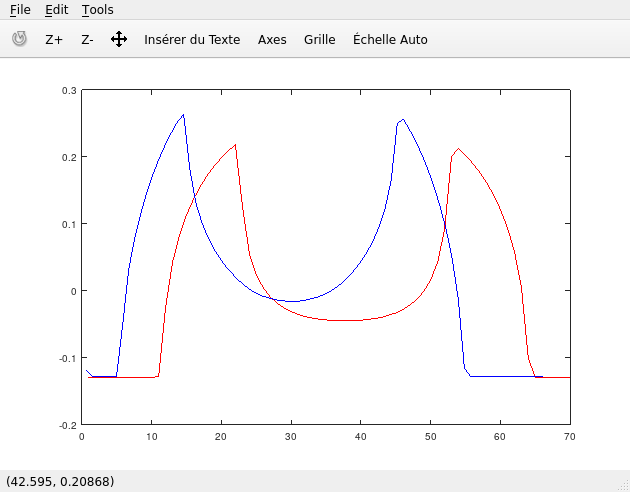
\includegraphics[width=0.35\textwidth]{../illus/comp/projO.png}
		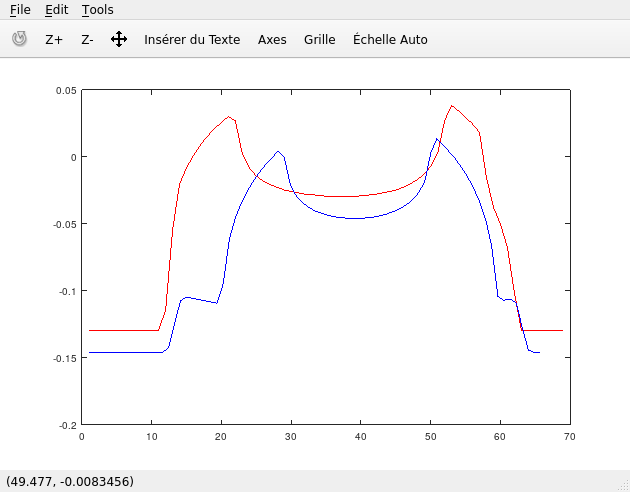
\includegraphics[width=0.35\textwidth]{../illus/comp/projS.png}\\
		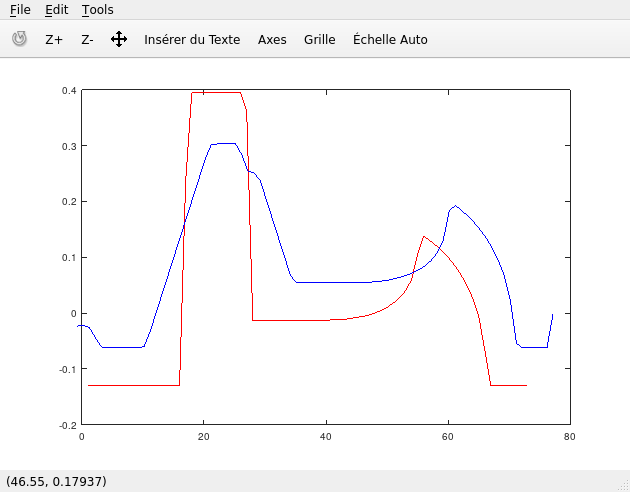
\includegraphics[width=0.35\textwidth]{../illus/comp/projP.png}
		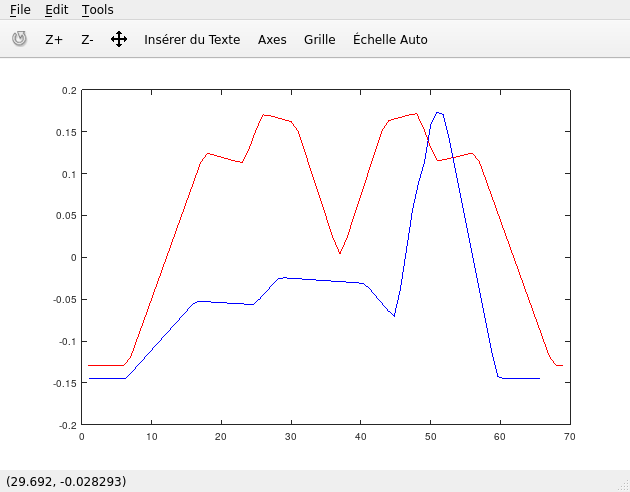
\includegraphics[width=0.35\textwidth]{../illus/comp/projA.png}
		\caption{Profil de certaines lettres: \texttt{O,S,P,A}, en rouge le normal et en blue l'italique}
	\end{figure}
	Pour certain caractère, c'est plus simple que pour d'autres.
	Un fois que la lettre est détéctée comme étant en \textit{italique}, on la redresse d'un certain coefficiant pour cela, on décale chaque ligne de pixel de plus en plus en exécutant le code suivant:
	\begin{lstlisting}[caption={Redressage de caractère dans Octave},language=Octave]
 for h=1:length(tile)-1
        tile(end-h,:)=[tile(end-h,1+round(h*length(tile(1,:))/(length(tile)*4.1)):end) tile(end-h,1:round(h*length(tile(1,:))/(length(tile)*4.1)))];
       endfor
\end{lstlisting}
		Cette fois dans le code \texttt{HTML}, on injecte une balise de type \textsl{<em>} en lui définissant le style, la couleur de la lettre, dans la balise.
\begin{lstlisting}[caption={Insertion d'un caractère italique dans Octave},language=Octave]
 predict=cstrcat("<em style='color:rgb(",num2str(colorL(1)),",",num2str(colorL(2)),",",num2str(colorL(3)),");'>",predict,"</em>");
\end{lstlisting}
		
	\subsection{Dimension}
	Le premier essais représentait le texte en police standard, minuscule sur la page web, nous avons donc décidé de gérer une notion de dimension des caractères. Pour cela, on se base sur la taille des tuiles de recherche. Plus la tuile est grande plus la police de caractère sur la page web sera grande.
\begin{lstlisting}[caption={Insertion de la couleur de fond dans Octave},language=Octave]
page=cstrcat("[..]<style>body{
background:rgb(",num2str(colorBG(1)),",",num2str(colorBG(2)),",",num2str(colorBG(3)),");
font-size:",num2str(dx_search*0.75),"px;
}</style>[..]");
\end{lstlisting}
	\section{Résultats}
	\paragraph{Couleurs}
	Figure \ref{coul}, on peut voir les résultats de notre script sur le fichier \texttt{Couleur.png}.
	\begin{figure}[h]
	\centering
		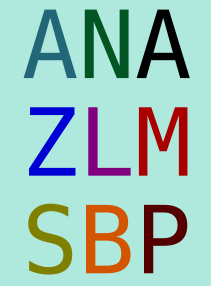
\includegraphics[height=0.2\textwidth]{../illus/Couleur.png}
		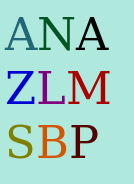
\includegraphics[height=0.2\textwidth]{../illus/CouleurR.png}
		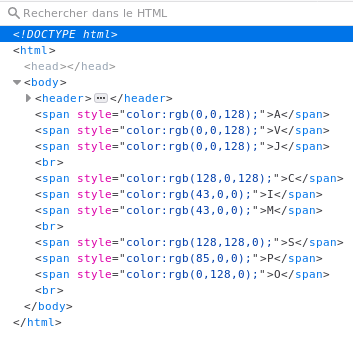
\includegraphics[height=0.2\textwidth]{../illus/CouleurC.png}
		\caption{Image, capture de la page web, capture du code}
		\label{coul}
	\end{figure}
	\paragraph{Gras}
Figure \ref{gras}, on peut voir les résultats de notre script sur le fichier \texttt{Gras.png}.
	\begin{figure}[h]
	\centering
		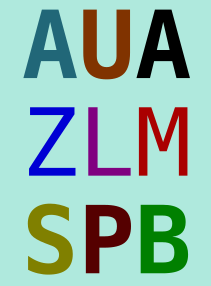
\includegraphics[height=0.2\textwidth]{../illus/Gras.png}
		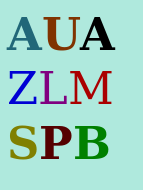
\includegraphics[height=0.2\textwidth]{../illus/GrasR.png}
		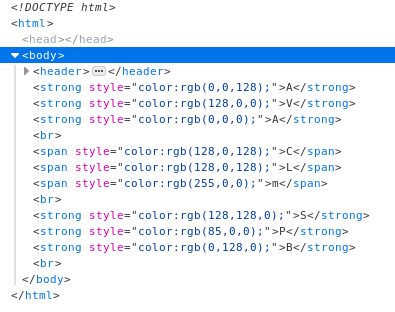
\includegraphics[height=0.2\textwidth]{../illus/GrasC.png}
		\caption{Image, capture de la page web, capture du code}
		\label{gras}
	\end{figure}
	\paragraph{Italique}
	Figure \ref{it}, on peut voir les résultats de notre script sur le fichier \texttt{Italique.png}.
	\begin{figure}[!h]
	\centering
		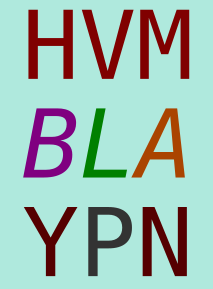
\includegraphics[height=0.2\textwidth]{../illus/Italique.png}
		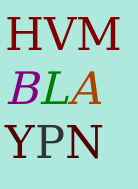
\includegraphics[height=0.2\textwidth]{../illus/ItaliqueR.png}
		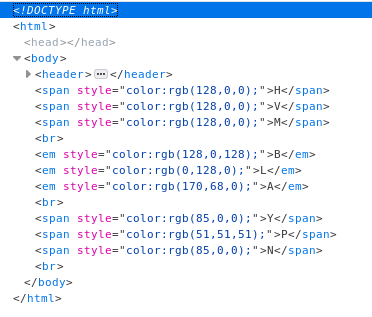
\includegraphics[height=0.2\textwidth]{../illus/ItaliqueC.png}
		\caption{Image, capture de la page web, capture du code}
		\label{it}
	\end{figure}
	\paragraph{Mix Total}
	Figure \ref{mix}, on peut voir les résultats de notre script sur le fichier \texttt{Mix.png}.
	\begin{figure}[!h]
	\centering
		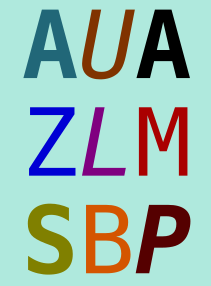
\includegraphics[height=0.2\textwidth]{../illus/Mix.png}
		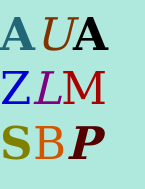
\includegraphics[height=0.2\textwidth]{../illus/MixR.png}
		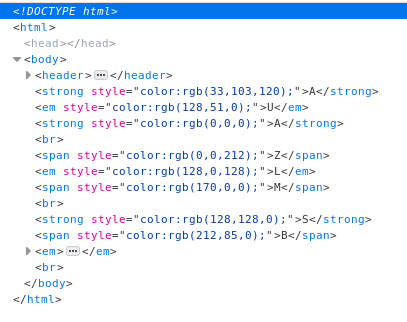
\includegraphics[height=0.2\textwidth]{../illus/MixC.png}
		\caption{Image, capture de la page web, capture du code}
		\label{mix}
	\end{figure}
	\subsection{Limitations}
	Les performances de notre script sont très limités. Chaque image présente des spécificités qui rendent la détection compliquée. Le script actuel est optimisé pour les majuscules et surtout pour les fichiers images tests fournis, le script fonctionne avec d'autres images mais les résultats ne seront pas parfait, avec par exemple des faux italiques, gras ou caractères. 
	On peut voir sur cet exemple que des caractères ne sont plus détecté ou que des faux styles apparaissent.
	\begin{figure}[!h]
	\centering
		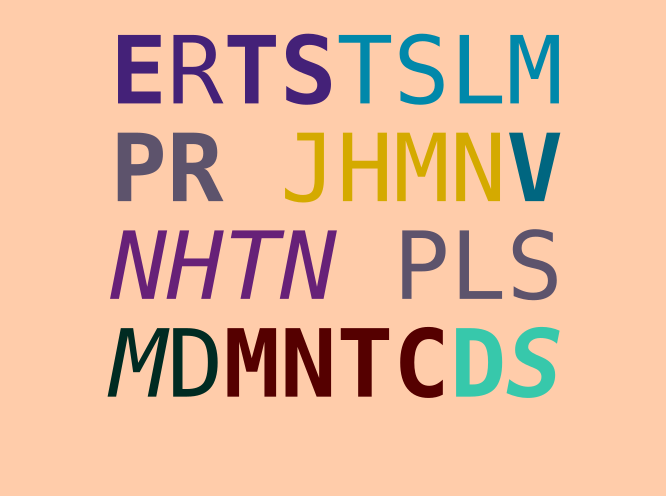
\includegraphics[height=0.25\textwidth]{../illus/CRASH.png}
		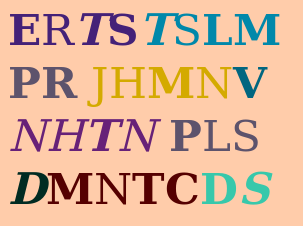
\includegraphics[height=0.25\textwidth]{../illus/fail.png}
		\caption{Image et capture de la page web}
	\end{figure}
	\section{Conclusion}
	Au fur et à mesure que le projet avancé, nous avons réussi à détecter de plus en plus d'éléments textuel et hypertextuel sur les images. Même si l'italique reste encore problématique, nous avons réussi à remplir les principaux objectifs.
	Le script que nous avons réalisé n'est pas le plus optimal il détecte relativement souvent des \textit{faux}, en effet la corrélation n'est pas le plus puissant et le plus optimisé des outils pour réaliser ce travail.
	De plus de nombreuses améliorations seraient encore à rajouter, comme par exemple la gestion de différentes tailles de caractères ou même de différentes polices.
	\listoffigures
	
	\lstlistoflistings
\end{document}